\documentclass[lettersize,journal]{IEEEtran}
\usepackage{amsmath,amsfonts}
\usepackage{algorithmic}
\usepackage{algorithm}
\usepackage{array}
\usepackage[caption=false,font=normalsize,labelfont=sf,textfont=sf]{subfig}
\usepackage{textcomp}
\usepackage{stfloats}
\usepackage{url}
\usepackage{verbatim}
\usepackage{graphicx}
\usepackage{cite}
\hyphenation{op-tical net-works semi-conduc-tor IEEE-Xplore}
% updated with editorial comments 8/9/2021
% For the documentation the IEEE Article Templates for Journals was used.

\begin{document}

\title{Generating handwritten numbers and letters using Conditional Generative Adverserial Nets}

\author{\textbf{Aszódi Zsombor, Babos Dávid, Kovács Gergely}\\
Deep Learning in Practice with Python and LUA\\
Faculty of Electrical Engineering and Informatics\\
Budapest University of Technology and Economics
}


\maketitle

\begin{abstract}
We propose a project for generating handwritten numbers and letters with Conditional Generative Adverserial Nets using the MNIST [1] and EMNIST [2] databases. The two main aims of the project is to create readable characters and to create the correct corresponding character for the embedded labels. Therefore with the help of an applied web interface the user can create handwritten characters corresponding to their input.
\end{abstract}


\section{Introduction}
The porpuse of the project is to get to know and apply both the theory and the structural integrity of cGANs, while creating a network, that is capable of image generation.
The main milestones of the project are the followings. 

Successfully importing the MNIST and EMNIST databases and preprocessing the data to the desired format.
Creating a Generative Adverserial Net (GAN) for the MNIST database.
Converting the GAN into a Conditional GAN (cGAN).
Trying an object orientated approach for model creation.
Creating a second cGAN model for the EMNIST letters database based on the previous model.
Optimizing hyperpatameters and testing the model.
Creating a web interface with the trained models.


\section{Generative Adverserial Nets}
The idea of GANs were first proposed by Ian J. Goodfellow and his colleagues in 2014 [3]. Since then GANs spread worldwide and have gained significant importance in the field of machine learning and artificial intelligence due to their ability to generate realistic and high-quality data. The basic idea behind GANs is to train two models simultaniously. The first model is a generative model, usually referred to as \textit{Generator}, and the other one is a discriminative model, the \textit{Discriminator}. The input of the \textit{Generator} is a noise vector, also called as a latent vector and the output is a generated image, called a fake image. The \textit{Generator} aims to capture the data distribution and tries to maximize the probability of the \textit{Discriminator} making a mistake. In other words the \textit{Generator} is trying to fool the \textit{Discriminator} into thinking that the generated fake image came from the training dataset. The \textit{Discriminator} tries to estimate the probability that a sample came from the training dataset rather than the \textit{Generator}. The two models are constantly fighting with each other, hence the name \textit{Adverserial}. The framework of GANs corresponds to a minmax two-player game.

\newpage

The upcoming figure illustrates a basic GAN model.\newline
\textit{[Figure 1 was retrieved from [5].]}

\begin{figure}[h]
    \centering
    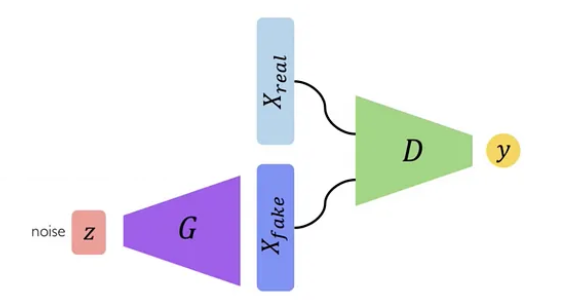
\includegraphics[width=10cm]{GAN_layout}
    \caption{Generative Adverserial Network [5]}
    \label{fig_1}
\end{figure}



\section{Conditional Generative Adverserial Nets}
The conditional version of GANs were introduced by Mehdi Mirza and Simon Osindero in late 2014 [4].\  Conditional GANs can be constructed by simply feeding the data, which we want to condition on, to both the \textit{Generator} and the \textit{Discriminator}. The condition used can be any kind of auxiliary information, such as class labels or data from other modalities. Conditioning is usually achieved by concatenating the input with an additional layer. In the generator the latent vector and the contition are combined/concatenated in joint hidden representation.

\vspace*{1em}The following figure illustrates the layout of a simple cGAN.\newline
\textit{[Figure 2 was retrieved from Mehdi Mirza's and Simon Osindero's work of Conditional Generative Adverserial Nets [4].]}

\begin{figure}[h]
    \centering
    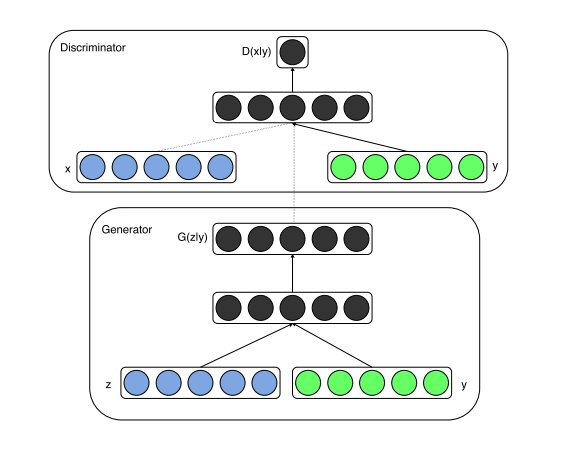
\includegraphics[width=10cm]{CGAN_layout}
    \caption{Conditional Generative Adverserial Network [4]}
    \label{fig_2}
\end{figure}
\newpage



\section{The importance of GANs}
In the following section we concluded why GANs are important and why we decided to work with them. There are some of the fields of machine learning and artificial intelligence, in which GANs play a major role in.

\begin{itemize}
    \item{\textbf{Data Generation:} GANs can generate synthetic data that closely resambles real data. This is peculiarly useful in situations where obtaining large quantities of labeled training data is challenging or expensive.}
    \item{\textbf{Super-Resolution:} GANs can enhance the resolution of images, enabeling the generation of high-quality images from low-resolution inputs. This is beneficial in fields such as medical imaging and analysis, or satellite image analysis.\ \textit{[6], [7], [8]}}
    \item{\textbf{Image Synthesis:} GANs are commonly used for image generation and synthesis tasks, including the generation of animals, human faces, and objects. This has applications is numerous fields such as computer vision, entertainment, and in recent years began to appear in the fields of art.}
    \item{\textbf{Style Transfer:} GANs can be employed for style transfer, allowing the transformation of images or videos to adopt the artistic style of another source. This has various forms of application in photo editing, video production, and artistic expression.\ \textit{[9]}}
\end{itemize}


\section{The MNIST Model}

The discriminator model takes a 28$\times$28 grayscale image, where each pixel has a value between -1 \& 1 as the input and outputs a binary prediction as to whether the image is real \textit{(class=1)} or fake \textit{(class=0)}.

Moreover a new second input is defined, which takes the class label of the image as an integer. This has the effect of making the input image conditioned on the provided class label.

Then the class label is passed through an Embedding layer. After hyperparameter optimization the size of the Embedding layer was set to 10. This basically means that a map of different 10-element vector representations are created for each of the 10 classes for the MNIST dataset. This representation will be learned by the discriminator model.

The output of the Embedding layer is than passed to a Fully Connected layer. Then the activations are reshaped into a single 28$\times$28 activation map and concatenated with the input. Hence it is important for the Fully Connected layer to have enough activations to be reshaped into one channel of a 28$\times$28 image. To conclude it has the effect of looking like a two-channel input image to the following Convolutional layer(s).


\vspace*{1em}The model is implemented as a convolutional neural network and we were trying to employe the model with the best possible practices for GAN design [12]. It uses the Adam version of stohastic gradient descent with a learning rate of 0.0002 and a momentum (beta) value of 0.5 [11].

As [11] suggests we tried using the leaky rectified activation function \textit{(Leaky ReLu)}, but with our model it resulted with poor and unstable loss values. Hence the model uses the \textit{Tanh} activation, which tourned out to produce stable results. The output layer uses the \textit{Sigmoid} activation function.

\vspace*{1em}The generator takes a point in the latent space as its input and creates a single 28$\times$28 size grayscale image as output. The model must be updated to take the class label. This has the effect of making the point in latent space conditioned on the class label.

A Fully Connected layer is used to interpret the point in latent space and to provide the needed activations that can be later reshaped into copies of a low-resolution version of the output image. The image version was determined to be of 7$\times$7 resolution and the layer creates 96 copies of it.

Similarly to the discriminator the following layer is an Embedding layer, which maps a unique 10-element vector for the class label.

The 10-element vector for the class labels is also passed through the Fully Connected layer and being resized into a single 7$\times$7 feature map to match the created image resolution. This new feature is then added to the existing features resulting in 97 feature maps.

Then the feature maps are upsampled twice using Transpose Convolutional layers. It results in the doubling of the size and quadrupling of the area of the activations.

\vspace*{1em}Unfortunately [11]'s suggestion to ReLu activation functions in the generator produced poor resultes. Therefore the \textit{Tanh} activation was used again, because it had better results.

Likewise to the discriminator the generator uses the Adam version of stohastic gradient descent with a learning rate of 0.0002 and a momentum (beta) value of 0.5 [11].

\vspace*{1em}For GAN models the use of Batch Normalization is highly recommended. But as [11] states if Batch Normalization is directly applied to all layers, it results in model instability and oscillating samples. This can be avoided by not applying Batch Normalization to the generator output layer and the discriminator input layer.

However with Batch Normalization applied the discriminator model became too strong compared to the generator and was able to estimate the probability that a sample came from the training dataset rather than the generator, with approximately a 100\% accuarcy. Therefore the generator could not obtain information sufficiently enough to fool the discriminator. When applied for only the generator it still resulted in model unstability. Hence the Batch Normalization layers were removed from the generator and were not used during the training of the discriminator.

\vspace*{1em}After the creation of the two separate models the main cGAN model is created. This model combines the discriminator and the generator and is responsible for the appropriate training method of the models. When the generator is trained it is important to turn off discriminator training and vice versa.

The cGAN model takes a point in latent sapce and a class label as inputs and generates a prediction of whether the input was real or fake.

For the model it is important to explicitly connect the class label - which was the input to the generator - and also the generator's generated image output, both as input to the discriminator. Thus functional API was used in the design of the model. This method allows the same class label to be the input for the generator and the discriminator as well.




\section{The EMNIST letters Model}

The second model, which works on the EMNIST letters dataset is mostly the same as the previous one, but it had been tuned to work on more input classes.
The major difference of the models is that the MNIST model had been applied with methods for observing and logging the metrics for evaluation of the generated images. Therefore it became possible to do hyperparameter optimization based on the metrics. The obtained hyperparameters from the MNIST model were used during the training of the EMNIST letters model as well.





\section{Metrics for evaluating generated images}
When evaluating generated images, the goal is to use an automatically computable metric to similarly characterize images as humans do. Some commonly used solutions are available for this purpose. In the unconditioned case, there are two conventional solutions, the Inception Score (IS) and the Fréchet Inception Disctance (FID).

Both use a pre-trained classifier to evaluate the generated images. For this purpose, the Inception V3 deep convolutional neural network is most commonly used. We cannot use this directly for the MNIST dataset, as we can only provide images of inappropriate size for its input. In this case the inputs can be rescaled. The classes on the output are also not appropriate, as they are trained on the ImageNet dataset. In the case where we are not using the output of the classifier fully connected layer, this is not a problem. However, in the case of the inception score, this output is required, in which case the classifier needs to be replaced and fine-tuned. An alternative, which was also used in [10], is to train a separate model instead of the Inception model and use it to compute the metrics.

\vspace*{1em}We chose this solution to use a very small and quickly computable model for validation, thus speeding up the process. The classifier is a simple convolutional neural network with convolutional layers, max pooling and batch normalization. The parameters were varied to keep the model size as small as possible while maintaining the highest possible accuracy on the test data. The accuracy of the model used for evaluation was above 99\%  on the dataset.

\begin{figure}[h]
    \centering
    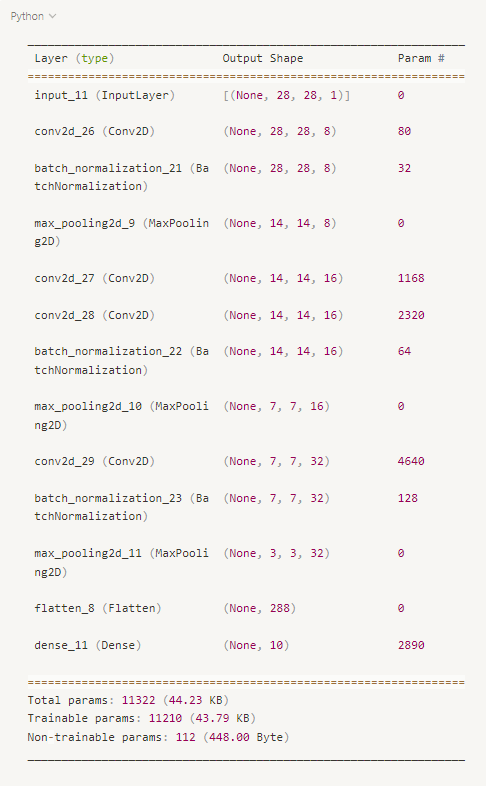
\includegraphics[width=8cm]{model}
    \caption{Model parameters for the model used for data evaluation}
    \label{fig_3}
\end{figure}
\newpage

In the conditional case IS is not sufficient, hence we used the between-class inception score (BCIS) and the within-class inception score (WCIS), which generalize the inception score, proposed in [10].

\vspace*{1em}For the conventional inception score, a classifier is used to estimate the conditional distribution of labels over generated images. In case of high quality images this distribution should have a low entropy, i.e., the classifier should predict high probability for one class. Due to the requirement of varied outputs, the marginal distribution should have a high entropy. To summarize these conditions, we use Kullback-Leibler (KL) divergence.

\begin{equation}
    IS(X;Y) := \text{exp} \{ \mathbb{E}_{x \sim D_G}[D_{KL}(p_G(y|x)||p_G(y))]\},
\end{equation}

In the conditioned case, BCIS calculates IS on the class averages. First, the outputs of the classifier are averaged over the samples in a conditioned class, and then the IS is calculated between them. For high BCIS samples in a conditioned class must clearly belong to one class, and all classes must cover the possibilities evenly.

\begin{align}
    BCIS(X;Y):&= IS(C;Y)\\
    &= \text{exp} \{ \mathbb{E}_{C \sim D_G}[D_{KL}(p_G(y|C)||p_G(y))]\}
\end{align}

WCIS calculates IS within classes. "It is a measurement of the mutual information between the
real classes conditioned on the samples and the real classes conditioned on the conditioned classes". High WCIS means wide variety inside a conditioned class.
\begin{equation}
    WCIS(X;Y) := \text{exp} \{\mathbb{E}_{C}[I(X_C;Y_C)]\},
\end{equation}
\begin{equation}
    I(X_C;Y_C) = \mathbb{E}_{x \sim D^e_G}[D_{KL}(p_G(y|x)||p_G(y|c))]
\end{equation}

\section{Hyperparameter optimization}
The metrics used for evaluation enable hyperparameter optimization to be performed based on them. For this purpose the KerasTuner framework was chosen, in which we experimented with the RandomSearch and Hyperband algorithms.

\vspace*{1em}We want to minimize the WCIS and maximize the BCIS metric. Calculating these metrics on the MNIST dataset yields a high BCIS around 9 and WCIS around 1. It took roughly 40 minutes per 10 epochs to train our CGAN network with a batch size of 32. For this time we ran the RandomSearch algorithm for the case of 10 parameter sets.

\vspace*{1em}The minibatch size had a significant impact on the trainnig process, since the small minibatch size meant more learning steps per epoch. We ran RandomSearch separately for each batch size. The batch size of 32 showed recognizable digits after a few epochs, while in case of 128 real images in a batch longer time was needed for similar results.

\vspace*{1em}We found that training duration is one of the most important factors influencing the quality of images. Within 8 epochs, the evaluation metrics did not change significantly, making it challenging to draw conclusions about the optimal hyperparameters based on these experiments. The conditioning labels matched the generated image only in a small proportion of cases. The parameter set chosen for the longer training was the run named smooth-rain-160, in which case the generated images were of the highest quality.

\begin{figure}[h]
    \centering
    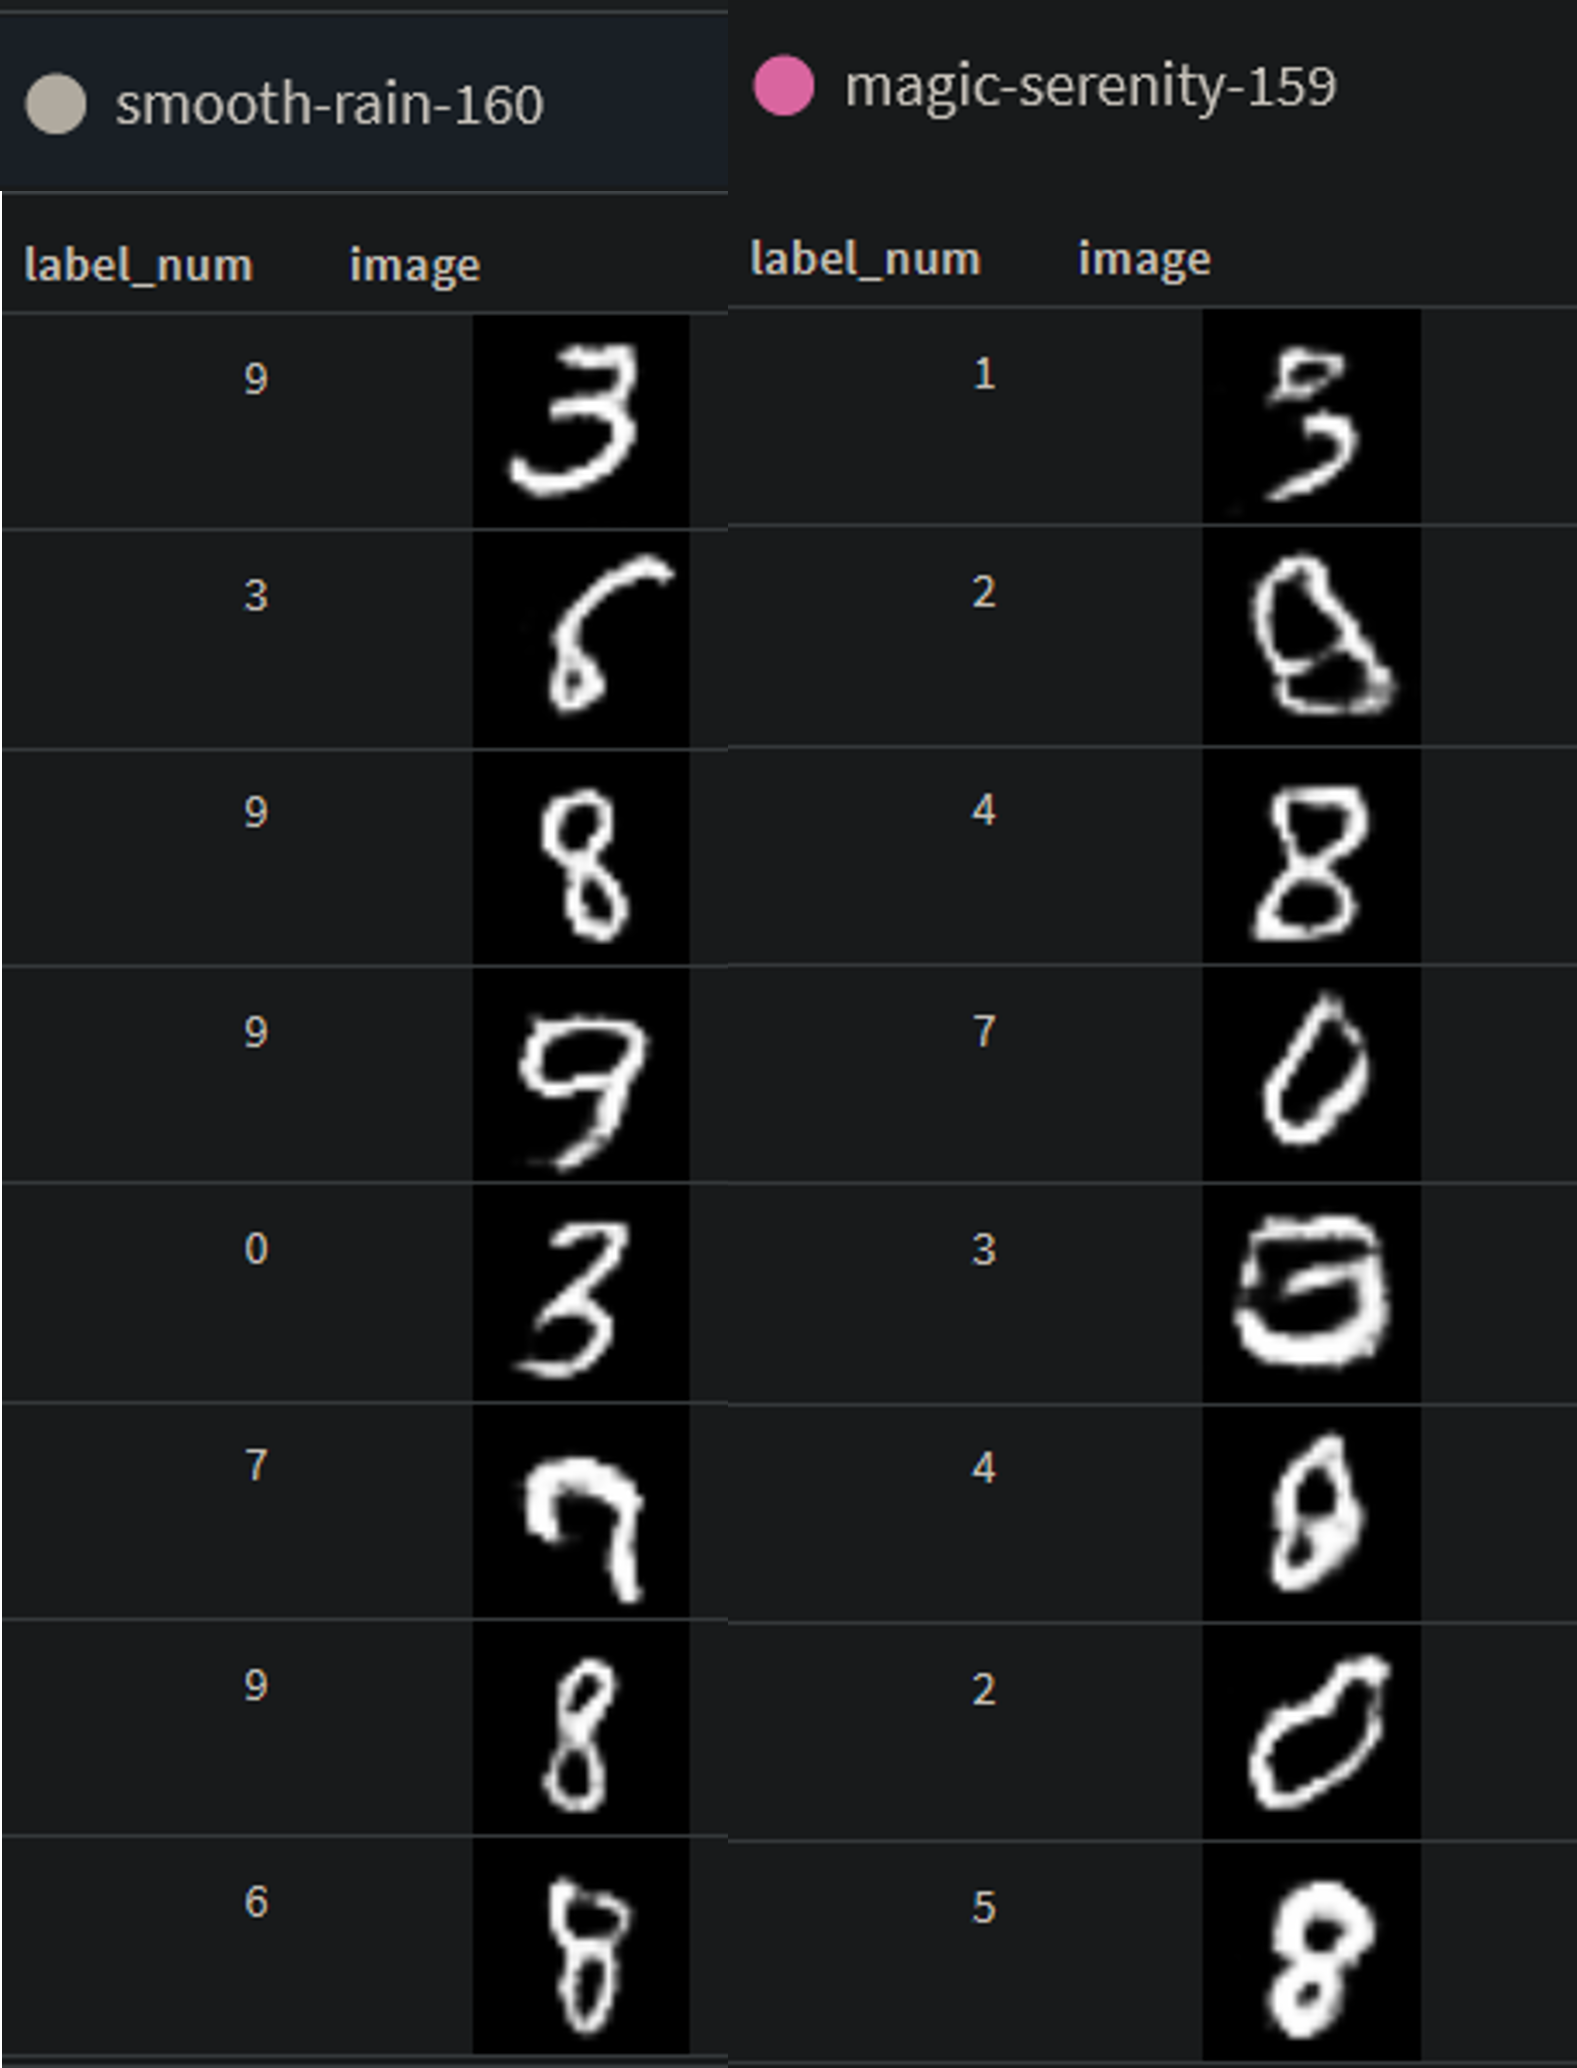
\includegraphics[width=8cm]{gen_images_cmp.png}
    \caption{Comparison of the generated images after hyperparameter optimization with RandomSearch}
    \label{fig_4}
\end{figure}

The stoic-resonance-155 run, demonstrating an outstandingly low WCIS value, generated examples exclusively with the digit 1.

\begin{figure}[h]
    \centering
    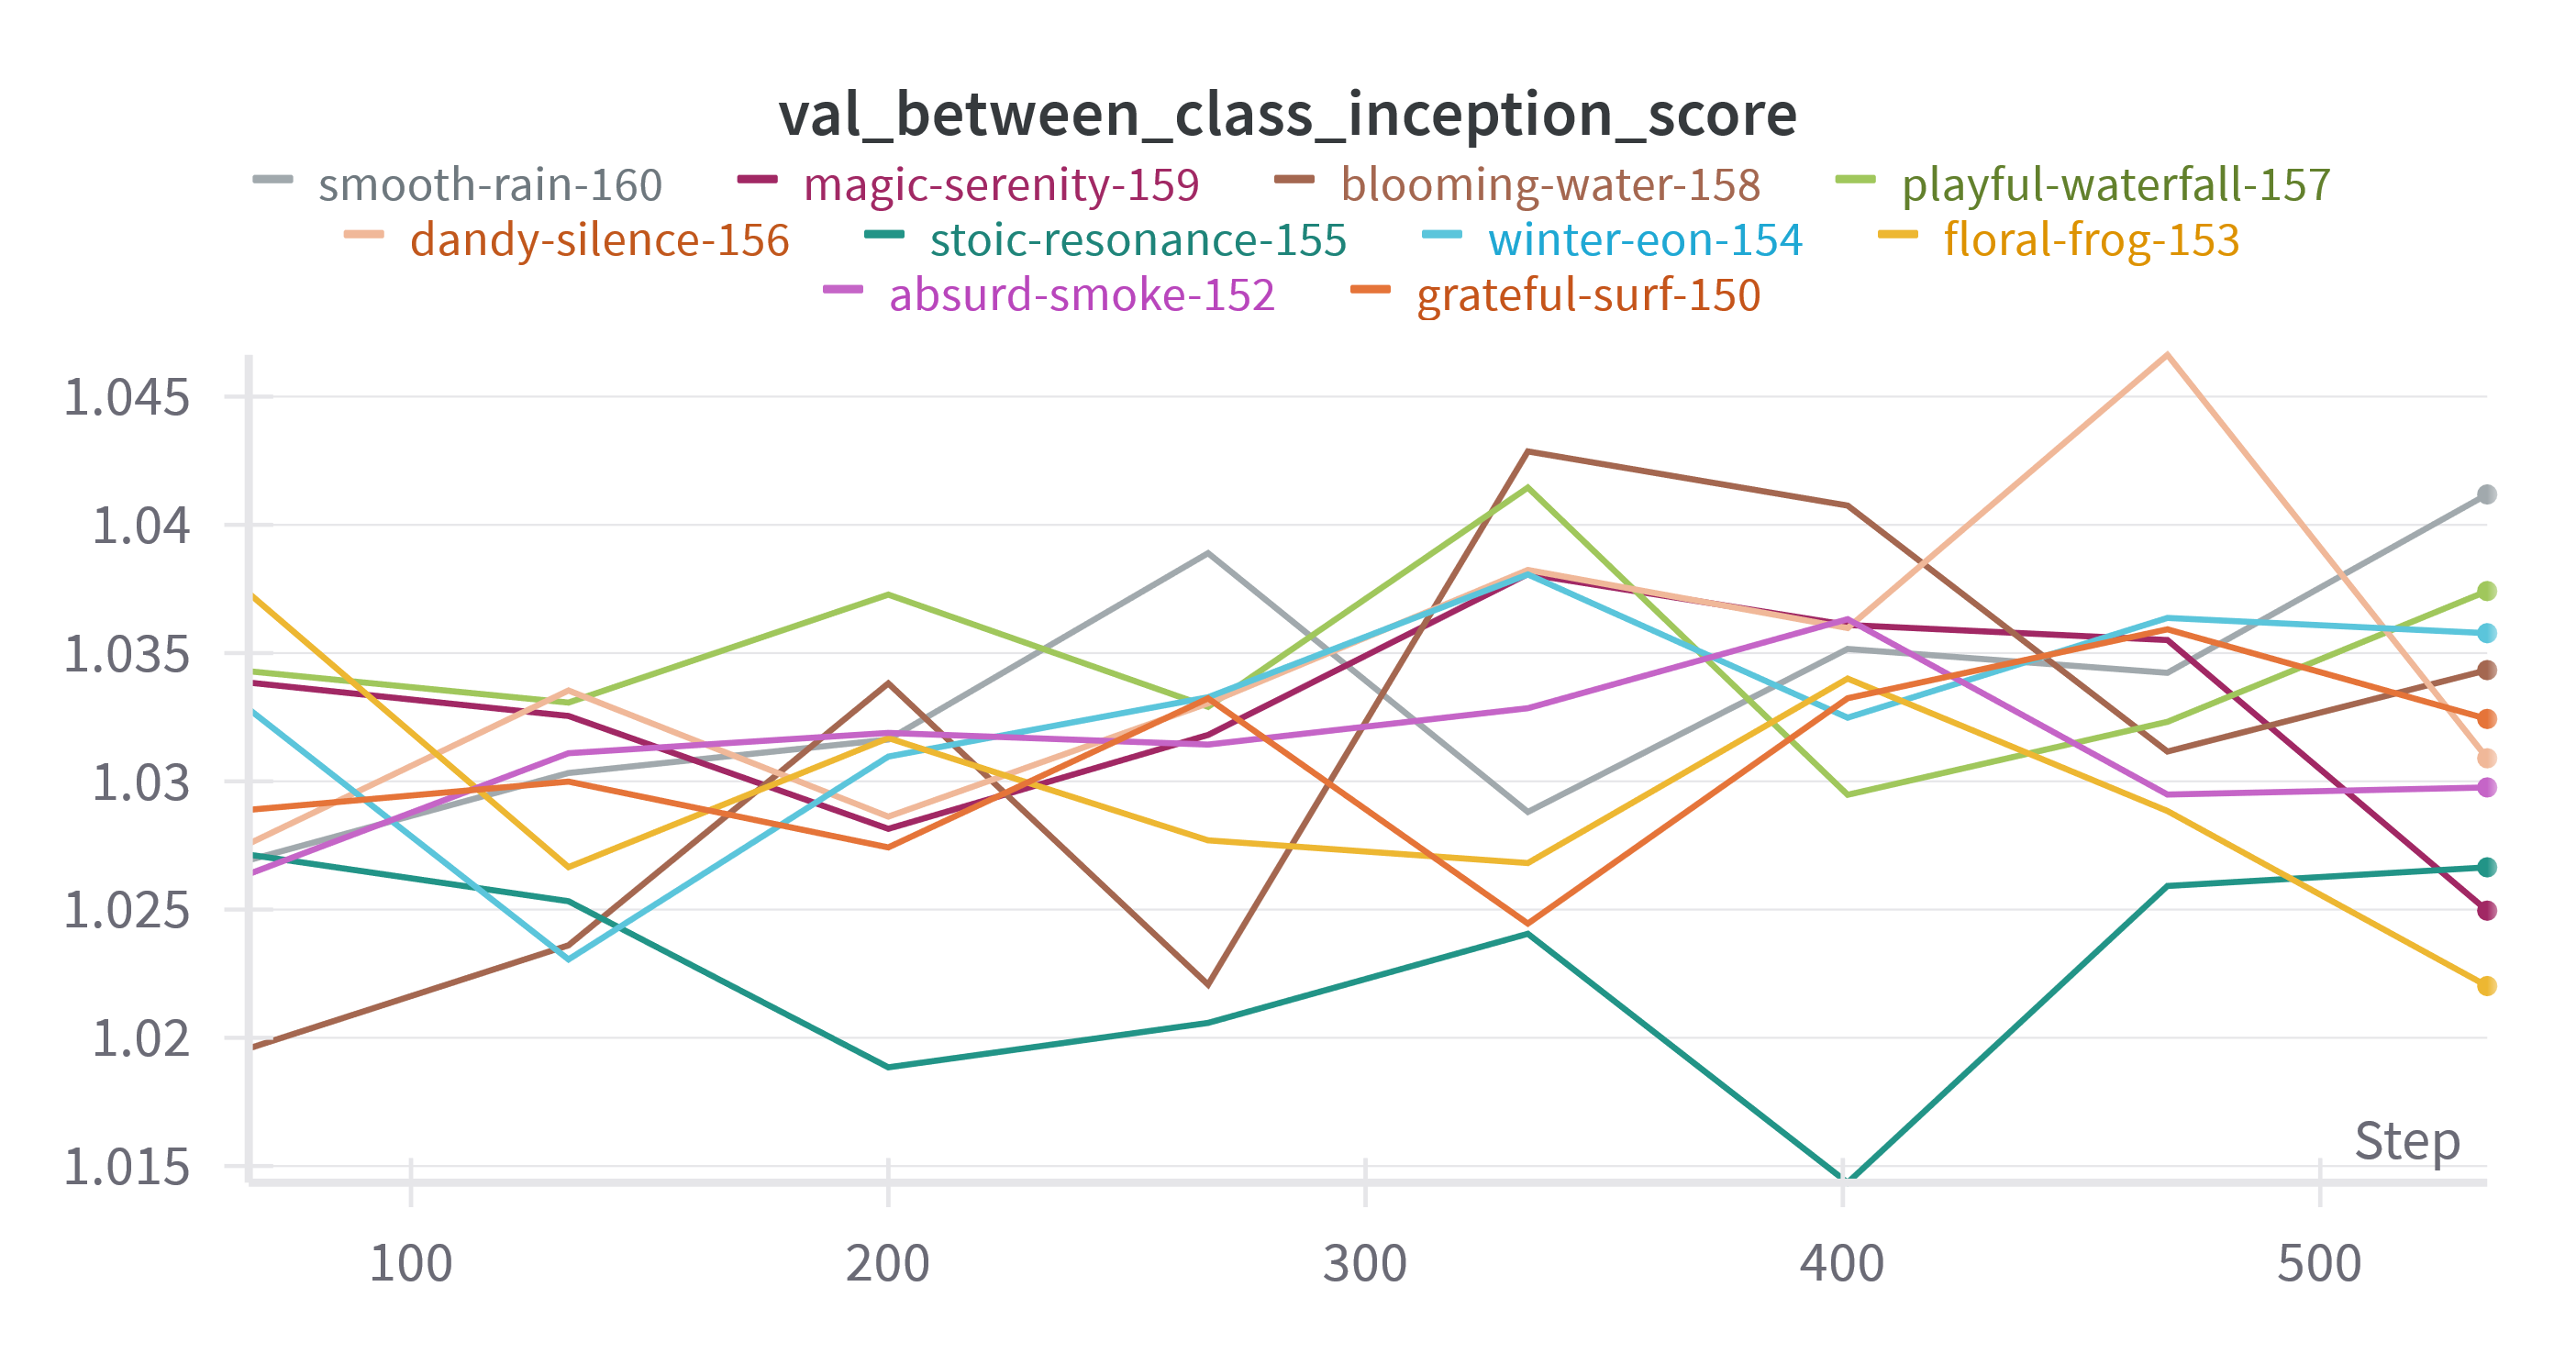
\includegraphics[width=9cm]{wnb_min_bcis.png}
    \caption{BCIS metric during hyperparameter optimization}
\end{figure}
\newpage

\begin{figure}[h]
    \centering
    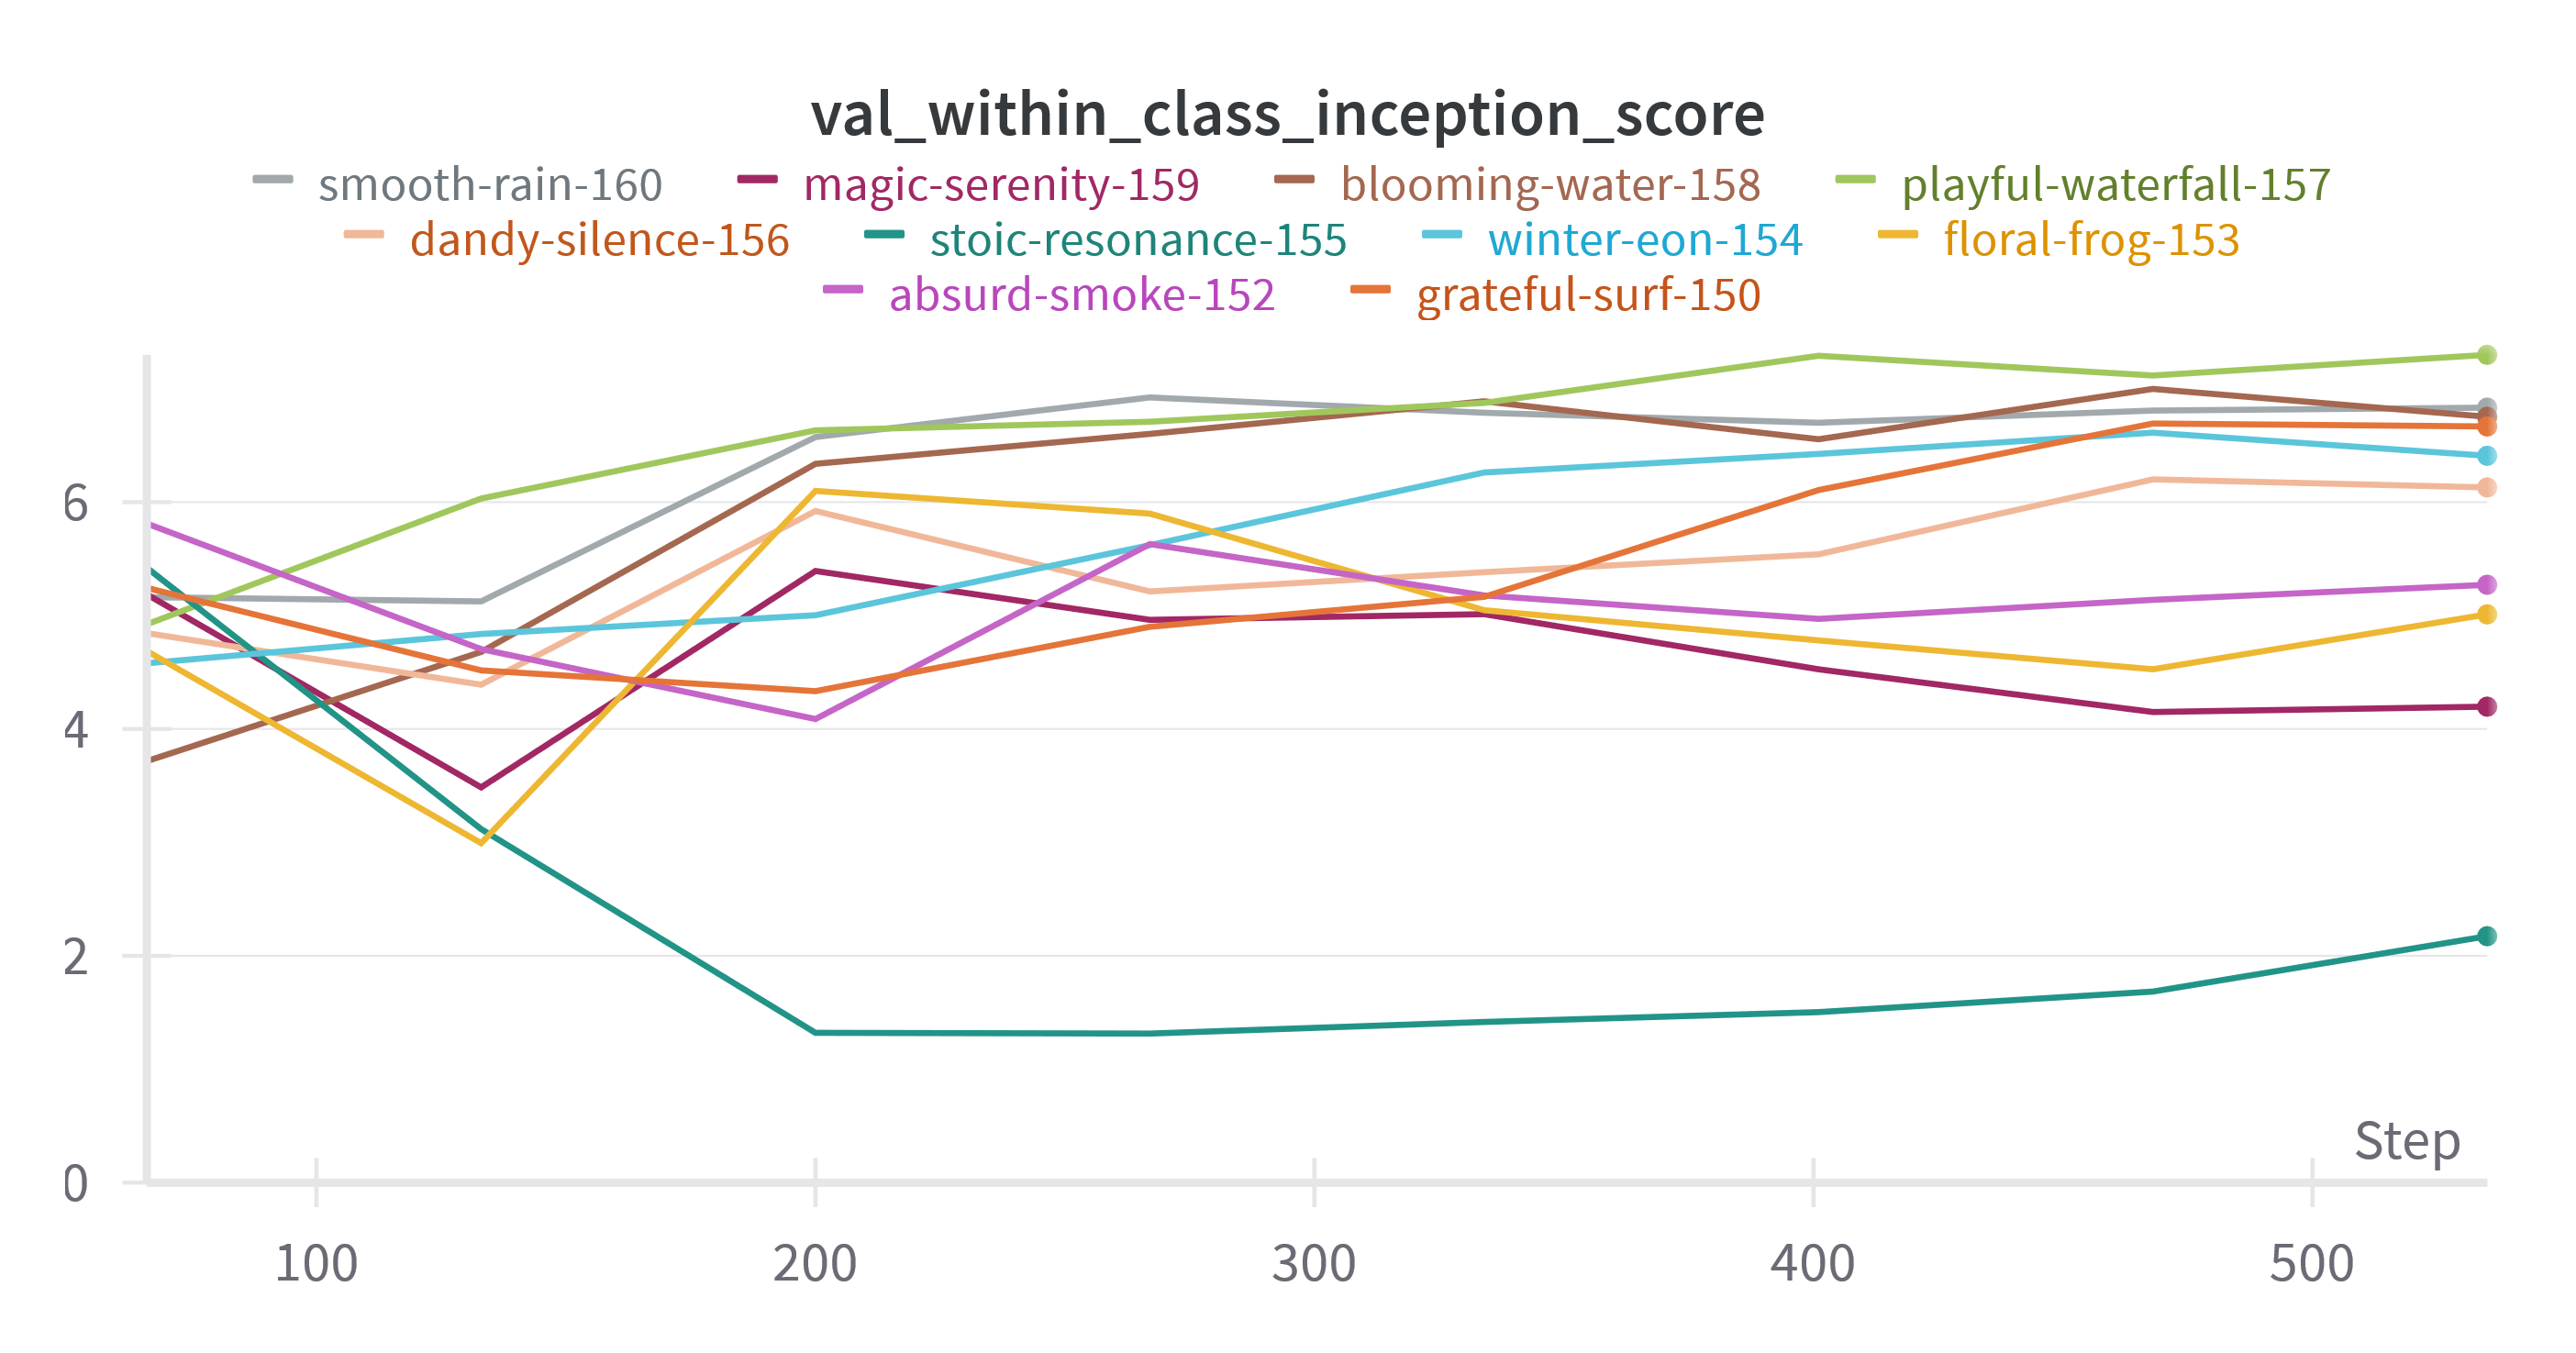
\includegraphics[width=9cm]{wnb_min_wcsi.png}
    \caption{WCIS metric during hyperparameter optimization}
\end{figure}


Since we found that the training time is one of the most important aspects for the model, a large number of epochs in the order of 100s are needed for convergence. But we did not have sufficient resources to run such trainings repeatedly to compare hyperparameters, we ran the best case selected from the hyperparameter searching experiments.

\section{Web Interface and Deploy Models}
After the models have been trained, it is important that they are made available to users in some form. In the role of an image-generating AI, this can be done in the form of a mobile app or even a website. Since a web interface is much more accessible to the majority of people nowadays, the model was deployed to a website. However, it is important that users do not have direct access to the model and that their devices do not have to be overloaded. Therefore, we will install it on a server and the communication will be done through the network by calling RestAPIs. The server runs two models, one responsible for generating handwritten digits and the other for generating handwritten letters. Once the API receives a request, it is checked by a regex to ensure that no model receives input that it is unable to process. Once the prompt has been accepted, the input is parsed and processed into a format that the generators can accept. During the prediction, we get images that are merged by a merging algorithm and serve as a final image. We save this on the server and give the access path as a response to the RestAPI. The web page can load and display the path received in the response.

\begin{figure}[h]
    \centering
    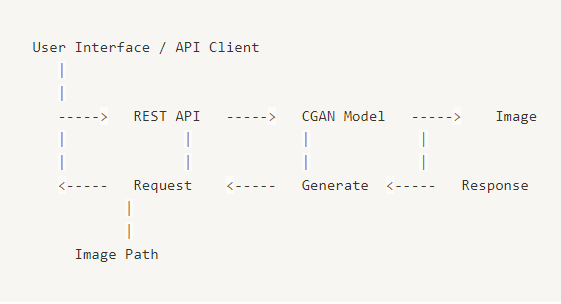
\includegraphics[width=9cm]{deploy_layout.png}
    \caption{The layout of the user interface}
\end{figure}
\newpage

\begin{figure}[h]
    \centering
    
\includegraphics[width=9cm]{web_api.png}
    \caption{RESTful API [13]}
\end{figure}

\section{Conclusion \& Results}
During the creation and test running of the model we encountered several problems about insufficient learning and memory usage. Thus we constructed the model in an object orientated form for favorable resource consumption. With this approach we were able to ward off the problems about great memory usage, but the runtime of the training increased.
Furthermore working with such great sized models is challenging. It is hard to train them using online platforms such as Google Colaboratory or Kaggle, due to long training time and large number of needed epochs.

One of the problems encountered during training the cGAN network was the failure to maintain a balance between the generator and the discriminator. The accuracy of the discriminator gradually increased, and the generator was not able to generate adequate samples. This may be related to the other significant factor, that the generator could not generate the conditioned classes properly, the labels did not match the generated images even after longer training.

It can be seen from the presented metrics below that the quality of the generated images did not increase either without (IS) or with (WCIS, BCIS) the tags being taken into account.

\begin{figure}[h]
    \centering
    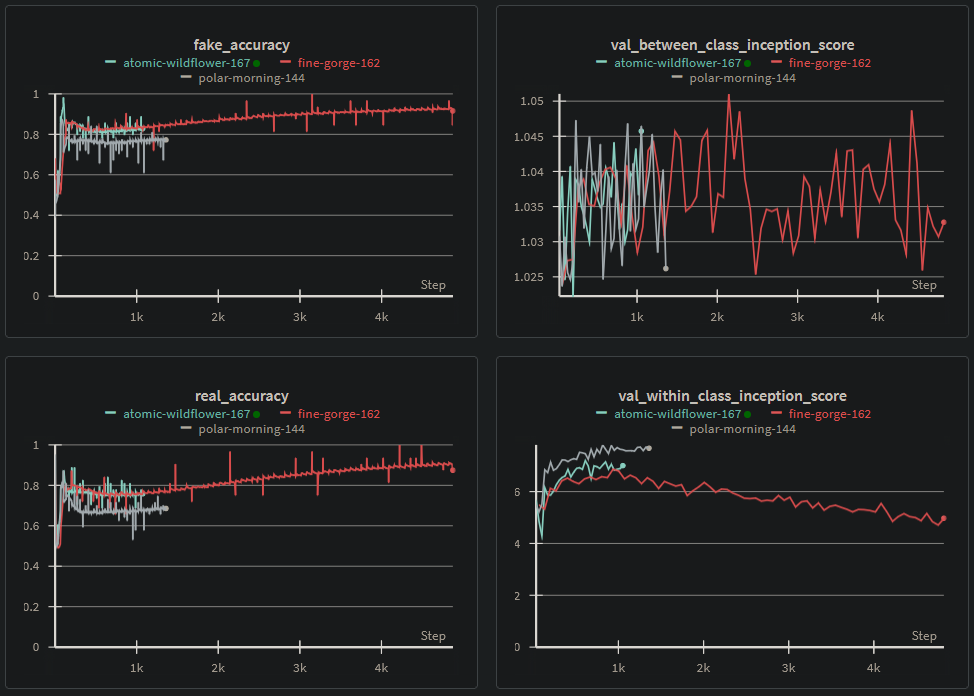
\includegraphics[width=9cm]{Untitled.png}
    \caption{The training process of the final model.}
\end{figure}

Samples were taken from the model during the training process. These were plotted later and were used in the determination of the best model along with the metrics.
\newpage

\begin{figure}[h]
    \centering
    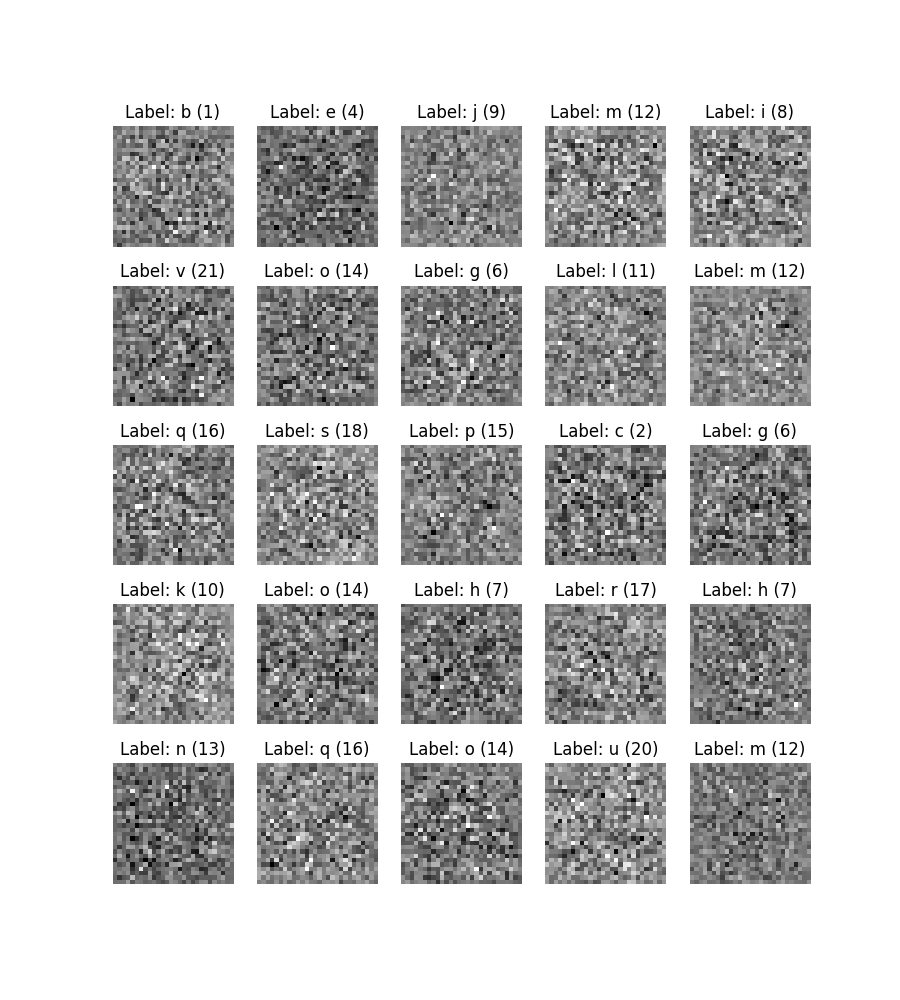
\includegraphics[width=5.5cm]{noise.png}
    \caption{At the beginning of the training}
\end{figure}
\begin{figure}[h]
    \centering
    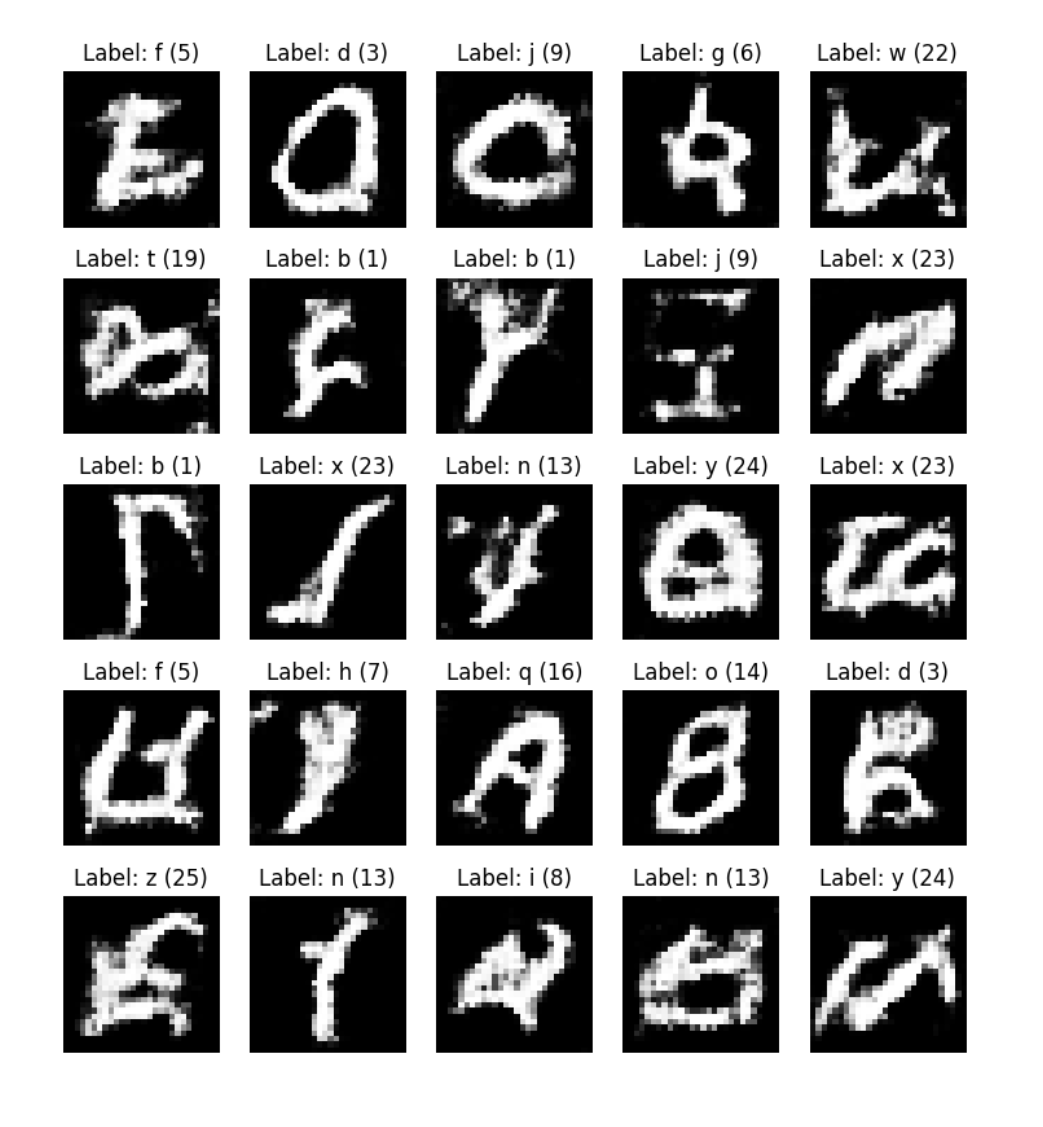
\includegraphics[width=5cm]{learning.png}
    \caption{In the middle of the training}
\end{figure}
\begin{figure}[h]
    \centering
    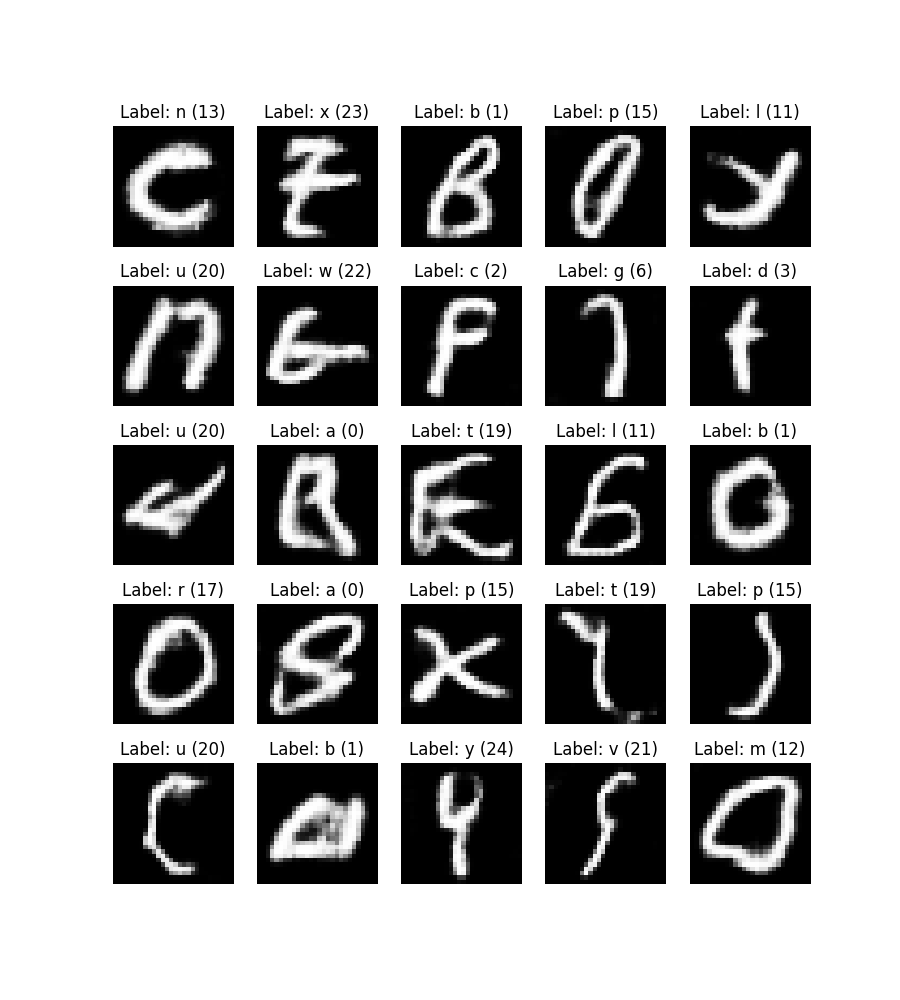
\includegraphics[width=5.5cm]{correct.png}
    \caption{At the end of the training}
\end{figure}

\newpage

\begin{figure}[h]
    \centering
    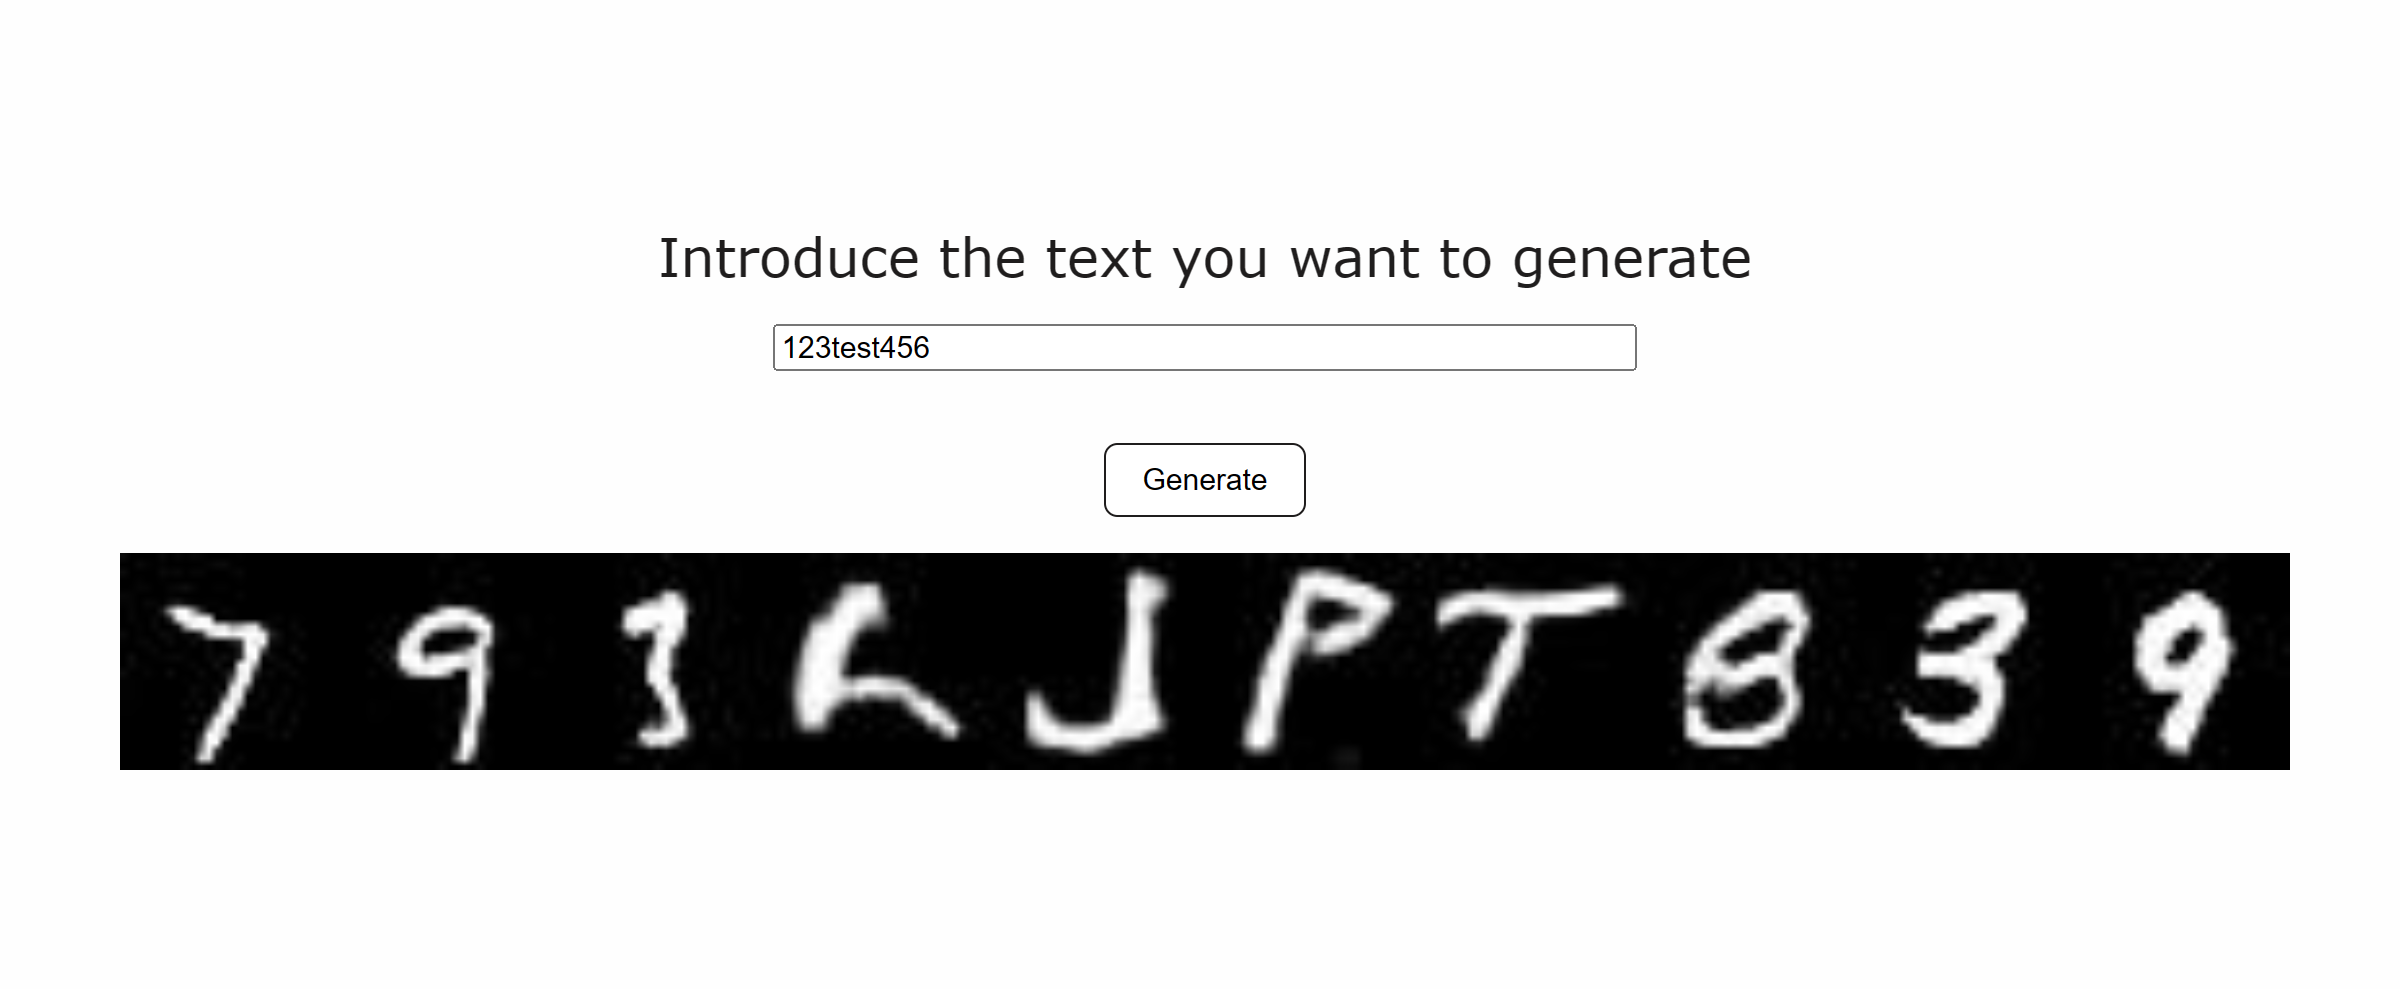
\includegraphics[width=9cm]{app.png}
    \caption{The user interface in action.}
\end{figure}


\section{Future plans}
Solving the issue of wrong character creation and creating the correct corresponding character for the actual label. This could be achieved with longer training times and modifying the arthitecture or with the use of diffusion models. Expanding the second model to train on the whole EMNIST database.


\section*{Acknowledgments}
This project was created within the Deep Learning in Practice with Python and LUA subject at Budapest University of Technology and Economics.


\begin{thebibliography}{1}
\bibliographystyle{IEEEtran}

\bibitem{ref1}
"THE MNIST DATABASE of handwritten digits". Yann LeCun, Courant Institute, NYU Corinna Cortes, Google Labs, New York Christopher J.C. Burges, Microsoft Research, Redmond. Retrieved from:\ http://yann.lecun.com/exdb/mnist/

\bibitem{ref2}
Cohen, G., Afshar, S., Tapson, J., and van Schaik, A. (2017). EMNIST: an extension of MNIST to handwritten letters. Retrieved from http://arxiv.org/abs/1702.05373

\bibitem{ref3}
Goodfellow, I. J., Pouget-Abadie, J., Mirza, M., Xu, B., Warde-Farley, D., Ozair, S., Courville, A., \& Bengio, Y. (2014). Generative adversarial nets. In NIPS’2014.\ 	arXiv:1406.2661

\bibitem{ref4}
Mehdi Mirza, Simon Osindero. Conditional Generative Adversarial Nets.\ 	arXiv:1411.1784

\bibitem{ref5}
Paul-Emile Gras: How to generate realistic pictures with Deep Convolutional GANs?\ https://medium.com/dc-gan/how-to-generate-realistic-pictures-with-deep-convolutional-gans-328beb40c14


\bibitem{ref6}
Christian Ledig, Lucas Theis, Ferenc Huszar, Jose Caballero, Andrew Cunningham,
Alejandro Acosta, Andrew Aitken, Alykhan Tejani, Johannes Totz, Zehan Wang, Wenzhe Shi
Twitter (2017). Photo-Realistic Single Image Super-Resolution Using a Generative Adversarial
Network.\ arXiv:1609.04802

\bibitem{ref7}
Ancla Müller1, Moritz Hackstein, Maksim Greiner, Philipp Frank, Dominik J. Bomans, Ralf-Jürgen Dettmar and Torsten Enßlin (2018). Sharpening up Galactic all-sky maps with complementary data A machine learning approach.\ arXiv:1806.04161

\bibitem{ref8}
Tang, H., Chen, X., Liu, Y. et al. Clinically applicable deep learning framework for organs at risk delineation in CT images. Nat Mach Intell 1, 480-491 (2019).\ https://doi.org/10.1038/s42256-019-0099-z

\bibitem{ref9}
Leon A. Gatys, Alexander S. Ecker, Matthias Bethge (2015). A Neural Algorithm of Artistic Style\ arXiv:1508.06576

\bibitem{ref10}
Benny, Y., Galanti, T., Benaim, S., \& Wolf, L. (2021). Evaluation metrics for conditional image generation. International Journal of Computer Vision, 129, 1712-1731.

\bibitem{ref11}
Alec Radford, Luke Metz, Soumith Chintala (2015). Unsupervised Representation Learning with Deep Convolutional Generative Adversarial Networks.\ arXiv:1511.06434

\bibitem{ref12}
Massimiliano Lupo Pasini, Vittorio Gabbi, Junqi Yin, Simona Perotto, Nouamane Laanait (2021). Scalable Balanced Training of Conditional Generative Adversarial Neural Networks on Image Data.\ arXiv:2102.10485

\bibitem{ref13}
Figure 5 was retrieved from tibco.com - What is a RESTful API?

\end{thebibliography}


\newpage




\end{document}


